\chapter{Thermal and Environmental Control}
\label{ch:thermal_environmental_control}
\section{Subsystem Scope and Design Drivers}
\label{sec:tcs_scope}
The Thermal and Environmental Control subsystem is responsible for maintaining the aerobot components within their allowable temperature ranges while protecting exposed hardware from the harsh Venus environment. This includes thermal control of the gondola, payload, power system, ISRU equipment, sampling hardware, and selected balloon-envelope interfaces.
% In addition to heating and cooling, the subsystem must address chemical resistance, ultraviolet degradation, and long-duration environmental exposure.
The main design drivers are:
\vspace{-5pt}
\begin{itemize}[itemsep=1pt, parsep=1pt]
    \item long-duration operation in the Venus cloud layer
    \item convective heat exchange with the Venus atmosphere
    \item solar and infrared radiative exchange through the cloud deck
    \item local thermal control of most temperature-critical hardware
    \item low power consumption and high reliability over the mission lifetime
    \item sulfuric-acid aerosol exposure
\end{itemize}
\vspace{-10pt}
\section{Venus Thermal and Environmental Conditions}
\label{sec:venus_thermal_environment}

The aerobot operates where the thermal environment is driven by atmospheric convection, solar and cloud-scattered radiation, atmospheric infrared radiation, and strong altitude-dependent temperature variation \cite{IngersollPechmann1980_VenusHeatBalance}. The surrounding sulfuric-acid aerosol environment also affects the long-term stability of exposed coatings, seals, and thermal surfaces \cite{delitsky2023cloudchemistryvenus,Yavrouian2003}.

For preliminary sizing, thermal effects as convection, solar radiation, infrared radiation, coating properties are represented by a conservative shell temperature, \(T_{\mathrm{shell}} = T_{\mathrm{ambient}}\). This simplification is appropriate at the current stage because detailed geometry, surface optical properties, coating degradation, view factors, and local flow conditions are not yet fixed.

The conductive heat leak through the gondola wall to the inside is estimated as \cite{incropera2011heattransfer}:
\begin{align}
    \dot{Q}_{\mathrm{wall}} =
    \frac{k_{\mathrm{eff}} A_{\mathrm{ext}}}{L_{\mathrm{ins}}}
    \left(T_{\mathrm{shell}} - T_{\mathrm{int}}\right),
    \label{eq:q_wall_prescribed_shell}
\end{align}
where \(k_{\mathrm{eff}}\) is the effective insulation conductivity, \(A_{\mathrm{ext}}\) is the total external area, \(L_{\mathrm{ins}}\) is the insulation thickness, and \(T_{\mathrm{int}}\) is the internal gondola temperature. The effective conductivity includes conduction and radiative transfer within the insulation, so no separate internal radiation term is added.

Thermal bridges and modelling uncertainty are included using a preliminary heat-leak safety factor:
\begin{align}
    \dot{Q}_{\mathrm{leak}} =
    SF_{\mathrm{leak}} \dot{Q}_{\mathrm{wall}}.
    \label{eq:q_leak_sf}
\end{align}
At this stage, \(SF_{\mathrm{leak}}=2.0\), accounting for supports, bolts, harnesses, feedthroughs, inlets, insulation imperfections, and uncertainty.

If active cooling is required, the cooler electrical power and hot-side rejection load are estimated as
\begin{align}
    P_{\mathrm{cooler,elec}} =
    \frac{\dot{Q}_{\mathrm{cool}}}{COP},
    \qquad
    \dot{Q}_{\mathrm{hot,reject}} =
    \dot{Q}_{\mathrm{cool}} + P_{\mathrm{cooler,elec}}.
    \label{eq:cooler_power_rejection}
\end{align}
Because the rejected heat must ultimately be dissipated to the Venus atmosphere, whole-gondola active cooling is avoided unless required by component temperature limits.


\section{Worst Case Scenarios}
\label{sec:tcs_worst_case_scenarios}

Worst-case hot and cold scenarios are used for preliminary sizing. Both use the prescribed shell-temperature model, where external convection, solar radiation, and infrared radiation are represented by assuming the shell is at ambient temperature. The assumptions are summarized in \autoref{tab:tcs_hot_cold_cases} and target temperatures are taken from \autoref{tab:thermal_requirements}.
\begin{table}[H]
\centering
\caption{Preliminary hot and cold case thermal assumptions.}
\label{tab:tcs_hot_cold_cases}
\renewcommand{\arraystretch}{1.1}
\begin{tabular}{|p{7.0cm}|p{1.6cm}|p{1.8cm}|p{1.4cm}|}
\hline
\textbf{Parameter} & \textbf{Hot Case} & \textbf{Cold Case} & \textbf{Unit} \\
\hline
Atmospheric temperature, \(T_{\mathrm{atm}}\) & 80 & -10 & \(^{\circ}\mathrm{C}\) \\
\hline
Prescribed shell temperature, \(T_{\mathrm{shell}}\) & 80 & -10 & \(^{\circ}\mathrm{C}\) \\
\hline
Internal target/minimum temperature, \(T_{\mathrm{int}}\) & 40 & 0 & \(^{\circ}\mathrm{C}\) \\
\hline
Temperature difference, \(\Delta T\) & 40 & 10 & K \\
\hline
External gondola area, \(A_{\mathrm{ext}}\) & \multicolumn{2}{c|}{1} & \(\mathrm{m^2}\) \\
\hline
Effective insulation conductivity, \(k_{\mathrm{eff}}\) & \multicolumn{2}{c|}{0.025} & \(\mathrm{W/(mK)}\) \\
\hline
Insulation thickness, \(L_{\mathrm{ins}}\) & \multicolumn{2}{c|}{0.05} & m \\
\hline
Heat-leak safety factor, \(SF_{\mathrm{leak}}\) & \multicolumn{2}{c|}{2.0} & -- \\
\hline
\end{tabular}
\end{table}
The wall and factored heat leaks are calculated from
\begin{align}
    \dot{Q}_{\mathrm{wall}} =
    \frac{k_{\mathrm{eff}} A_{\mathrm{ext}}}{L_{\mathrm{ins}}}
    \Delta T,
    \qquad
    \dot{Q}_{\mathrm{leak}} =
    SF_{\mathrm{leak}}\dot{Q}_{\mathrm{wall}}
    \label{eq:q_wall_and_leak_case}
\end{align}
The resulting preliminary heat leaks are summarized in \autoref{tab:tcs_hot_cold_results}.
\begin{table}[H]
\centering
\caption{Preliminary hot and cold case heat-leak results.}
\label{tab:tcs_hot_cold_results}
\renewcommand{\arraystretch}{1.1}
\begin{tabular}{|p{5.2cm}|p{2.6cm}|p{2.6cm}|}
\hline
\textbf{Quantity} & \textbf{Hot Case} & \textbf{Cold Case} \\
\hline
Wall heat leak, \(\dot{Q}_{\mathrm{wall}}\) & 20 W & 5 W \\
\hline
Factored heat leak, \(\dot{Q}_{\mathrm{leak}}\) & 40 W & 10 W \\
\hline
Thermal effect & Heat input & Heat loss \\
\hline
\end{tabular}
\end{table}



An active cooler does not destroy this heat. It transfers heat from the internal gondola volume to the external side of the thermal system. In doing so, the cooler also consumes electrical power, which appears as additional heat that must be rejected to the surroundings. Therefore, the required cooler power is
\begin{align}
    P_{\mathrm{cooler,elec,hot}}
    =
    \frac{\dot{Q}_{\mathrm{cool,hot}}}{COP},
    \label{eq:p_cooler_hot}
\end{align}
where \(COP\) is the coefficient of performance of the cooling device. The total heat that must be rejected at the hot side is then a sum of external heat leak, heat generated by internal subsystems and heat from the cooler.
\begin{align}
    \dot{Q}_{\mathrm{hot,reject}}
    =40 + \dot{Q}_{\mathrm{internal,hot}}
    +
    P_{\mathrm{cooler,elec,hot}}.
    \label{eq:q_hot_reject_hot_case}
\end{align}
This means that whole-gondola active cooling is difficult in the Venus atmosphere: the system must not only remove the internal heat load, but also reject the cooler's own electrical power as additional heat. For this reason, active cooling is retained only for local high-temperature-critical hardware, while duty cycling and altitude adjustment (see \autoref{subsec:thermal_control_altitude_adjustment}) are preferred for reducing the total heat load.


\section{Thermal Control by Altitude Adjustment}
\label{subsec:thermal_control_altitude_adjustment}

The preliminary power estimates show that continuous active thermal control would exceed reasonable power limits, especially when there are zero power generation periods. Therefore, thermal control by altitude adjustment is proposed as a major operational contributor. Since the Venus atmospheric temperature changes by about 10 degrees Celsius per kilometer, the aerobot can reduce thermal control demand by moving to colder or warmer layers depending on the mission state. This may reduce power or even eliminate the need for active heating or cooling.

However, altitude adjustment cannot replace onboard thermal-control hardware. It may be too slow for fast transients and can be constrained by science operations, communication needs, buoyancy-system limitations, or failure cases. Therefore, passive and active thermal-control hardware is still required for redundancy, emergency operation, and local component protection. These hardware options are traded in the following sections.

% \section{Chemical Environment}
% \label{subsec:chemical_environment}
% The cloud-layer environment contains sulfuric-acid aerosols. This affects the thermal subsystem because exposed surfaces such as coatings may degrade over time. Thermal surfaces must therefore be selected not only for their initial absorptivity and emissivity, but also for their long-term stability after acid-aerosol exposure.


% -------------------------------------------------------------------------------

\section{Thermal and Environmental Control Subsystem Overview}

\subsection{Thermal Subsystem Requirements}
\label{sec:tcs_requirements}
The subsystem requirements are derived from the need to maintain critical components within their
allowable temperature limits while ensuring environmental compatibility. The preliminary
requirements are listed in \autoref{tab:tcs_requirements}.
\begin{table}[H]
\centering
\renewcommand{\arraystretch}{1}
\small
\caption{Preliminary thermal and environmental-control requirements.}
\label{tab:tcs_requirements}
\begin{tabular}{|p{2.5cm}|p{10.5cm}|}
\hline
\textbf{ID} & \textbf{Requirement} \\
\hline
REQ-TCS-01 & The TCS shall maintain all critical components within their survival temperature limits during all mission phases after deployment. \\ \hline
REQ-TCS-02 & The TCS shall maintain batteries, avionics, payload instruments, and sampling hardware within their operational temperature limits during required operating modes. \\ \hline
REQ-TCS-04 & The TCS exposed to sulfuric-acid aerosol shall retain required function after exposure. \\ \hline
REQ-TCS-05 & The TCS shall provide thermal monitoring for batteries, avionics, payload instruments. \\
\hline
\end{tabular}
\end{table}


%------------------------------------------------------------------------------
% \section{Thermal Model and Performance Metrics}
% \label{sec:tcs_model}

% At this stage, the thermal design is evaluated using a lumped-parameter energy balance. For each thermal node, the governing equation is

% \begin{align}
%     C \frac{dT}{dt}
%     =
%     \dot{Q}_{\mathrm{int}}
%     + \dot{Q}_{\mathrm{solar}}
%     + \dot{Q}_{\mathrm{IR}}
%     + \dot{Q}_{\mathrm{conv}}
%     - \dot{Q}_{\mathrm{loss}},
%     \label{eq:lumped_energy_balance}
% \end{align}

% where \(C\) is the thermal capacitance of the node, \(T\) is the node temperature, \(\dot{Q}_{\mathrm{int}}\) is internal heat dissipation, \(\dot{Q}_{\mathrm{solar}}\) is absorbed solar heat, \(\dot{Q}_{\mathrm{IR}}\) is absorbed infrared heat, \(\dot{Q}_{\mathrm{conv}}\) is convective exchange with the atmosphere, and \(\dot{Q}_{\mathrm{loss}}\) includes radiative, conductive, and convective heat losses.

% Thermal performance is quantified using the temperature margin. For a hot case, the margin is

% \begin{align}
%     M_{\mathrm{hot}} =
%     T_{\mathrm{max,allow}} - T_{\mathrm{hot,pred}} - U,
%     \label{eq:hot_margin}
% \end{align}

% and for a cold case,

% \begin{align}
%     M_{\mathrm{cold}} =
%     T_{\mathrm{cold,pred}} - T_{\mathrm{min,allow}} - U,
%     \label{eq:cold_margin}
% \end{align}

% where \(U\) is the thermal uncertainty allowance. A concept passes the thermal-performance criterion if all critical components have positive hot-case and cold-case margins.
%=--------------------------------------------------------------------------------

\subsection{Component Thermal Requirements}
\label{sec:component_thermal_requirements}
The TCS shall keep each critical component within its operational temperature range when active and within its survival range when inactive. For component \(i\), this is expressed as

\begin{align}
    T_{\mathrm{min,op},i} \leq T_i \leq T_{\mathrm{max,op},i},
    \qquad
    T_{\mathrm{min,surv},i} \leq T_i \leq T_{\mathrm{max,surv},i}.
    \label{eq:component_temperature_requirements}
\end{align}

At this stage, most preliminary temperature limits are assigned by component class and shall be replaced by manufacturer values during detailed design.

\begin{table}[H]
\centering
\small
\caption{Preliminary component-level thermal requirements for VISTA, based on typical spacecraft component temperature ranges \cite{wertz1999smad} and \autoref{tab:venus_payload}}
\label{tab:thermal_requirements}
\renewcommand{\arraystretch}{1}
\begin{tabular}{|p{6.8cm}|p{2.3cm}|p{2.3cm}|}
\hline
\textbf{Component / Zone} & \multicolumn{2}{c|}{\textbf{Temperature Ranges ($^\circ$C)}}  \\
\cline{2-3}
 & \textbf{Service} & \textbf{Survival}  \\
\hline

Battery pack / Batteries & 20 to 40 & 0 to 60 \\
\hline

Power electronics / Power Box Baseplates & -10 to 50 & -20 to 60  \\
\hline


C\&DH Box Baseplates & -20 to 60 & -40 to 75  \\
\hline


Solar Panels & -150 to 110 & -200 to 130  \\
\hline


Communication antennas / Antennas & -100 to 100 & -120 to 120  \\
\hline


Payload - NMS & -20 to 50 & TBD \\
\hline

Payload - AFN & -10 to 40 & TBD \\
\hline


Payload - WIS  & -40 to 60 & TBD \\
\hline


Payload - Sonic Anemometer & -40 to 50 & TBD \\
\hline


Payload - Barometers & -54 to 70 & TBD \\
\hline



Payload - mTLS & -40 to 80 & TBD \\
\hline


Payload - Pyrgeometer & -20 to 80 & TBD \\
\hline




Payload - TOPS & -20 to 50 & TBD \\
\hline


Payload - OPC & -50 to 50 & TBD \\
\hline




%===================================================================

% Avionics & TBD & TBD \\
% \hline

% Aerosol inlet and sampling line & TBD & TBD  \\
% \hline

% Sampling valves & TBD & TBD  \\
% \hline

% ISRU / gas-separation hardware & TBD & TBD  \\
% \hline

% Balloon envelope interface & TBD & TBD \\
% \hline


% External gondola shell & TBD & TBD \\
% \hline

\end{tabular}
\end{table}

The battery pack, power electronics and AFN are treated as thermally critical items, and are therefore used as upper and lower limits in \autoref{sec:tcs_worst_case_scenarios}.


%---------------------------------------------------
\subsection{Environmental Protection Subsystem Requirements}
\label{sec:environmental_protection_requirements}

The Environmental Protection part of the subsystem is responsible for preventing degradation of the gondola, exposed interfaces, thermal surfaces, and sensitive internal hardware due to the Venus cloud-layer environment. The main environmental hazards considered at this design stage are sulfuric-acid aerosols, atmospheric exposure, ultraviolet radiation, contamination of thermal-control surfaces, and long-duration material ageing.

The environmental protection requirements are listed in \autoref{tab:env_protection_requirements}.

\begin{table}[H]
\centering
\small
\caption{Preliminary environmental protection requirements.}
\label{tab:env_protection_requirements}
\renewcommand{\arraystretch}{1}
\begin{tabular}{|p{2.8cm}|p{10.5cm}|}
\hline
\textbf{ID} & \textbf{Requirement} \\
\hline
REQ-ENV-01 & Exposed external surfaces shall be compatible with sulfuric-acid aerosol exposure for the required mission duration. \\
\hline
REQ-ENV-02 & Sensitive electronics, batteries, avionics, and payload electronics shall be isolated from direct Venus atmospheric exposure. \\
\hline
REQ-ENV-03 & Environmental protection materials shall be compatible with the expected thermal range of the mission. \\
\hline
% REQ-ENV-05 & The aerosol sampling path shall be environmentally isolated from the main avionics and battery zones. \\
% \hline
\end{tabular}
\end{table}

\subsection{Component Environmental Protection Requirements}
\label{sec:component_environmental_protection_requirements}

Environmental protection is assigned according to exposure level. Internal electronics, batteries, avionics, and most payload hardware are protected by the sealed gondola. External surfaces, feedthroughs, sensors, aerosol inlets, and sampling lines require acid-compatible materials because they may directly contact the Venus cloud environment. The sampling path is treated as a high-risk interface because it intentionally exchanges material with the atmosphere and can create a contamination or leakage path into the gondola.
% Different components experience different levels of exposure to the Venus environment. Therefore, environmental protection is assigned by component or interface class rather than applying the same protection method to all hardware. Components located inside the sealed gondola require contamination control and external surfaces, sampling hardware, feedthroughs, and sensors require direct sulfuric acid compatibility.

% \begin{table}[H]
% \centering
% \small
% \caption{Preliminary component-level environmental protection requirements.}
% \label{tab:component_env_protection_requirements}
% \renewcommand{\arraystretch}{1}
% \begin{tabular}{|p{3.3cm}|p{3.2cm}|p{8.0cm}|}
% \hline
% \textbf{Component / Interface} &
% \textbf{Exposure Level} &
% \textbf{Environmental Protection Implication} \\
% \hline

% External gondola shell &
% Direct exposure &
% Requires acid-resistant outer surface, such as FEP, PTFE, PFA, or another verified acid-compatible coating or film. \\
% \hline

% Thermal coating / outer thermal surface &
% Direct exposure &
% Must retain thermal-optical properties after sulfuric-acid aerosol, UV, and thermal cycling exposure. Ordinary spacecraft white paints are not assumed acceptable without compatibility testing. \\
% \hline

% Structural shell &
% Protected or partially exposed &
% Should use corrosion-resistant metal or be fully protected by an external acid barrier. Bare aluminium is not preferred for exposed surfaces. \\
% \hline

% Insulation layer &
% Protected internal layer &
% Aerogel, microporous silica, or foam insulation shall be placed behind an acid-resistant outer barrier and shall not be directly exposed to Venus aerosols. \\
% \hline

% Feedthroughs and penetrations &
% High-risk interface &
% Require metal, ceramic-to-metal, or glass-to-metal feedthroughs where possible. Polymer seals should be minimized or backed up by secondary seals. \\
% \hline

% Aerosol inlet and sampling line &
% Intentional exposure &
% Requires acid-compatible materials and isolation from the main gondola volume. Candidate materials include PFA/PTFE-lined tubing, titanium, or Hastelloy-type fittings. \\
% \hline

% Sampling valves &
% Intentional or partial exposure &
% Require acid-compatible valve bodies, seals, and local thermal control to prevent condensation, clogging, or acid accumulation. \\
% \hline

% Payload electronics &
% No direct exposure &
% Should be placed inside the sealed gondola or protected instrument housing. Environmental protection is mainly through isolation and thermal control. \\
% \hline

% Batteries and avionics &
% No direct exposure &
% Must remain inside the sealed and thermally controlled gondola volume. Direct Venus exposure is not acceptable. \\
% \hline

% External sensors and optical windows &
% Direct exposure &
% Require acid-compatible housings and window materials. Sapphire, fused silica, or protected optical materials may be considered depending on sensor needs. \\
% \hline

% \end{tabular}
% \end{table}


\section{Design Option Tree}
\label{sec:tcs_dot}

The design option tree in \autoref{fig:TCStreeplaceholder} is divided into six top-level decision groups:
\begin{enumerate}[itemsep=1pt, parsep=1pt]
    \item Thermal Control System Architecture
    \item Gondola  Thermal Enclosure
    \item Thermal Zoning
    \item Environmental Protection
    \item Thermal Monitoring
    \item Thermal Control Subsystem
\end{enumerate}


\begin{figure}
    \centering
    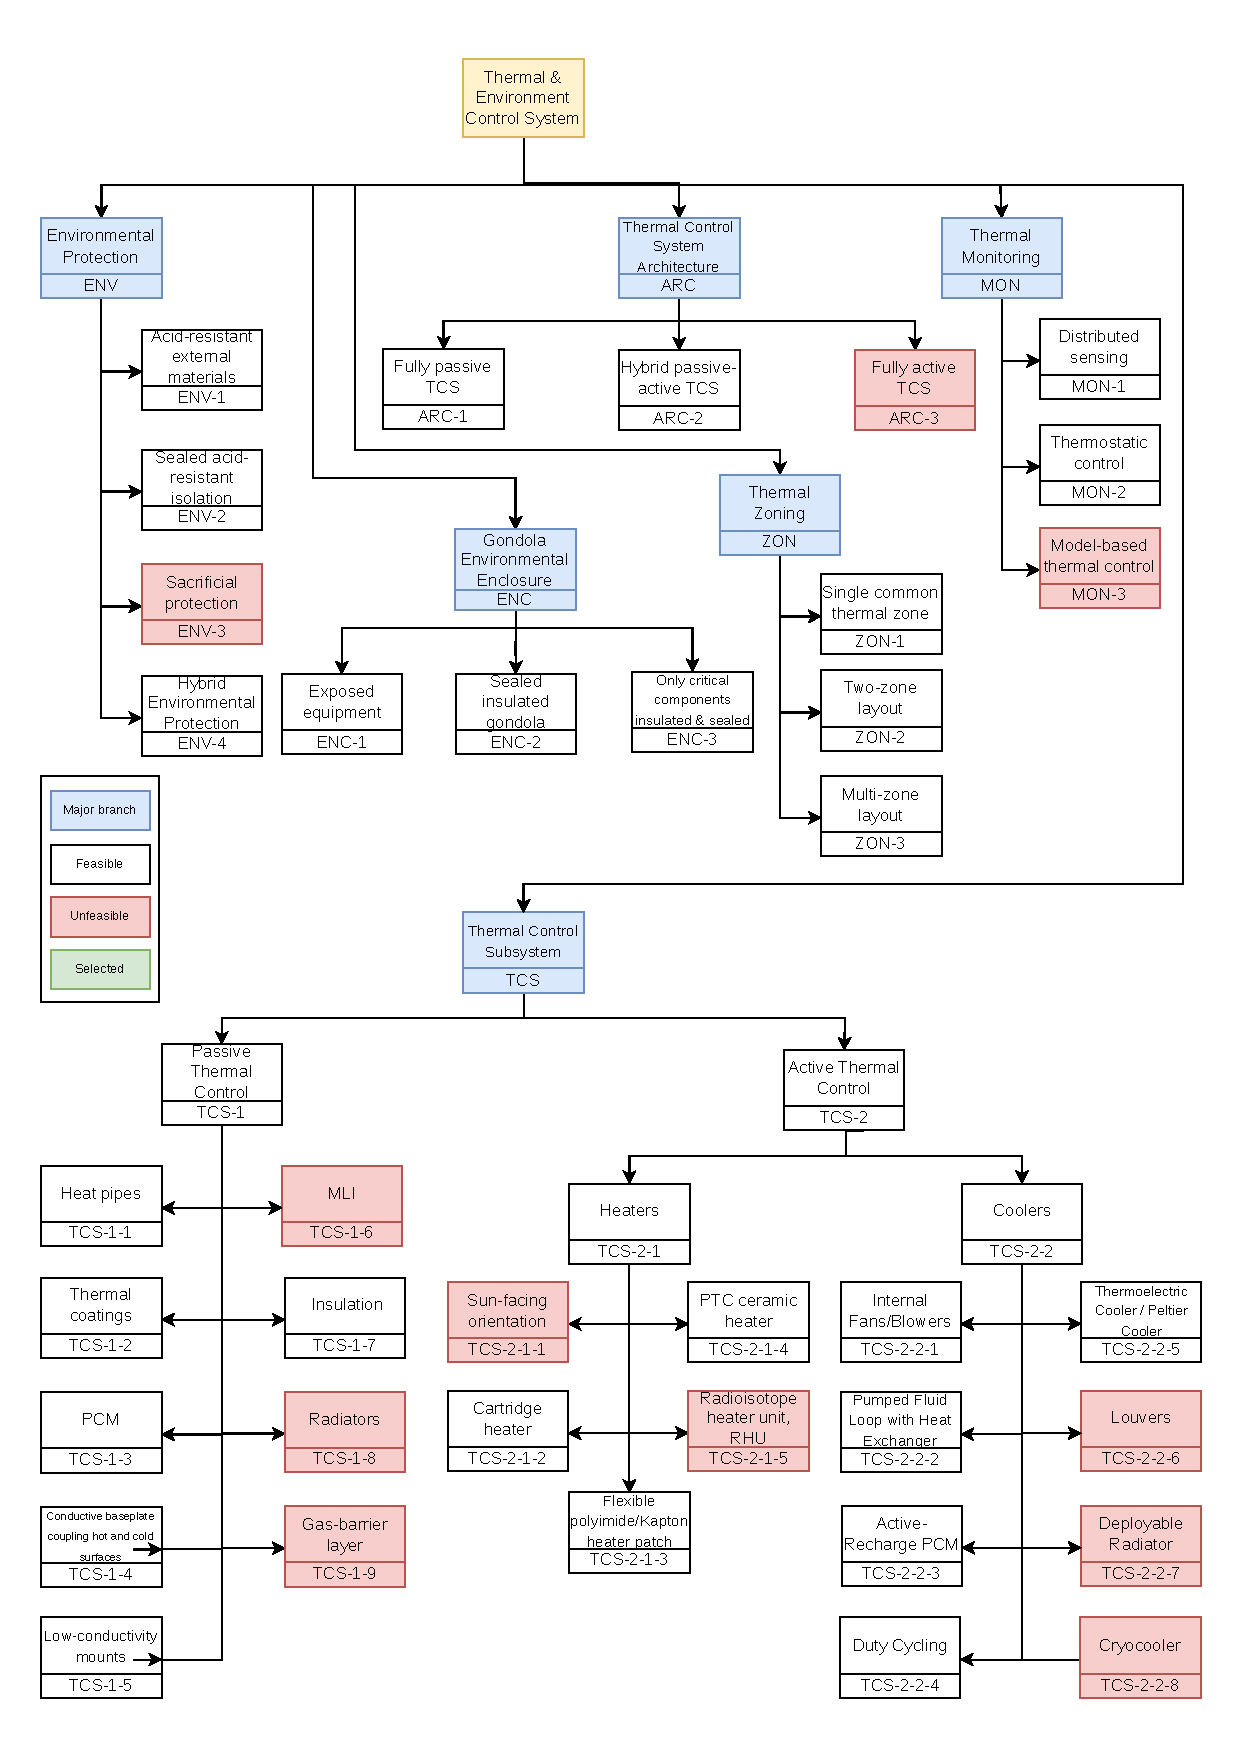
\includegraphics[width=1.0\linewidth]{fig/WFD-DOT_Th&Env.drawio.pdf}
    \caption{Thermal and environmental-control design option tree.}
    \label{fig:TCStreeplaceholder}
\end{figure}

\subsection*{Pruned Options}
\label{subsec:tcs_pruned_options}

The following options are removed before the trade-off procedure because they are incompatible with the constraints.

\begin{itemize}[itemsep=1pt, parsep=1pt]

\item \textbf{ARC-3 - Fully active TCS}: Rejected due to high mass, continuous power demand, and increased reliability risk compared with a passive-dominant hybrid architecture.

\item \textbf{ENV-3 - Sacrificial protection}: Rejected because degradation-based protection cannot guarantee stable environmental isolation over the full mission lifetime.

\item \textbf{MON-3 - Model-based thermal control}: Rejected at this stage because it requires a validated high-fidelity thermal model, more sensors, and more complex control logic.

\item \textbf{TCS-2-1-1 - Sun-facing orientation}: Rejected because the aerobot drifts with the Venus atmosphere and cannot rely on fixed orientation relative to the Sun.
\item \textbf{TCS-2-1-5 - Radioisotope heater unit, RHU}: Constant nuclear heating is not required and cannot be easily switched off. RHUs also introduce major safety, availability, integration, and regulatory constraints compared with simple electrical heaters.
\item \textbf{TCS-1-6 - MLI-based external insulation}: Rejected as primary external insulation because MLI is most effective in vacuum, while Venus atmospheric convection is expected to dominate heat transfer.

\item \textbf{TCS-2-2-6 - Louvers}: Rejected because external moving parts are difficult to seal and protect from sulfuric-acid aerosols over a long-duration mission.

\item \textbf{TCS-2-2-7 - Deployable radiator}: Rejected due to deployment risk, exposed moving interfaces, acid compatibility concerns, and limited heat-rejection benefit in the warm Venus atmosphere.

\item \textbf{TCS-2-2-8 - Cryocoolers}: Rejected because cryogenic temperatures are not required, and the mass, power demand, vibration, and complexity are not justified for ordinary electronics operating temperatures.

\end{itemize}
%------------------------------------------------------------------------
\section{Trade-Off}
\subsection{Trade-Off Method}

\label{sec:tcs_tradeoff_method}
Because the TCS consists of compatible hardware functions rather than one mutually exclusive architecture, the trade-off is performed in functional groups and then integrated into one selected concept. Architecture, enclosure, zoning, environmental protection, passive control, heating, and cooling options are compared separately using criteria relevant to each decision group.

A score from 1 to 5 is used for all trade-off criteria. A score of 1 indicates poor performance or major design risk, 3 indicates acceptable performance with concerns, and 5 indicates strong performance with low implementation risk.

\subsection{Candidate Architecture Tradeoffs}

\definecolor{score5}{RGB}{0,176,80}
\definecolor{score4}{RGB}{146,208,80}
\definecolor{score3}{RGB}{255,255,0}
\definecolor{score2}{RGB}{255,192,0}
\definecolor{score1}{RGB}{255,0,0}

% ============================================================
% ARCHITECTURE TRADE-OFF
% ============================================================

\subsection*{TCS method}

\begin{table}[H]
\centering
\normalsize
\caption{Thermal Control System architecture trade-off.}
\label{tab:tcs_architecture_tradeoff}
\renewcommand{\arraystretch}{1}
\setlength{\tabcolsep}{2pt}
\resizebox{\textwidth}{!}{%
\begin{tabular}{|p{1.3cm}|p{3.0cm}|p{4.0cm}|p{3.6cm}|p{3.6cm}|p{3.4cm}|p{3.6cm}|p{0.9cm}|}
\hline
\textbf{ID} &
\textbf{Option$\downarrow$ / Criteria$\rightarrow$} &
\textbf{Thermal Performance (30\%)} &
\textbf{Power Demand (25\%)} &
\textbf{Reliability (20\%)} &
\textbf{Mass / Complexity (15\%)} &
\textbf{Venus Environment Compatibility (10\%)} &
\textbf{Score} \\
\hline

ARC-1 &
\textbf{Fully passive TCS} &
\scorecell{2}{Limited control authority during hot and cold cases.} &
\scorecell{5}{No active thermal-control power required.} &
\scorecell{4}{Failure modes like surface degradation possible, but no moving parts.} &
\scorecell{5}{Lowest mass and simplest implementation.} &
\scorecell{1}{May not protect all sensitive hardware under harshest Venus conditions and throughout missions lifetime.} &
\textbf{3.5} \\
\hline

ARC-2 &
\textbf{Hybrid passive-active TCS} &
\scorecell{5}{Passive stability with local active correction where required.} &
\scorecell{3}{Active power needed only when required.} &
\scorecell{2}{Failure modes like surface degradation possible, but active elements can fail as well.} &
\scorecell{4}{Moderate mass and medium hardware count.} &
\scorecell{5}{Can adapt to Venus atmosphere variations and local component needs.} &
\textbf{3.75} \\
\hline

\end{tabular}%
}
\end{table}

% ============================================================
% GONDOLA ENCLOSURE TRADE-OFF
% ============================================================

\subsection*{Gondola Enclosure}
\begin{table}[H]
\centering
\normalsize
\caption{Gondola environmental enclosure trade-off.}
\label{tab:gondola_enclosure_tradeoff}
\renewcommand{\arraystretch}{1.25}
\setlength{\tabcolsep}{2pt}
\resizebox{\textwidth}{!}{%
\begin{tabular}{|p{1.3cm}|p{3.1cm}|p{4.4cm}|p{4.2cm}|p{3.8cm}|p{3.8cm}|p{0.9cm}|}
\hline
\textbf{ID} &
\textbf{Option$\downarrow$ / Criteria$\rightarrow$}&
\textbf{Environmental Isolation (35\%)} &
\textbf{Thermal Protection (35\%)} &
\textbf{Mass / Complexity (20\%)} &
\textbf{Integration, Simplicity (10\%)} &
\textbf{Score} \\
\hline

ENC-1 &
\textbf{Exposed equipment} &
\scorecell{1}{Sensitive equipment would be directly exposed to Venus atmosphere and acid aerosols.} &
\scorecell{1}{Poor protection from external convection and environmental temperature changes.} &
\scorecell{5}{Lowest mass and no enclosure hardware.} &
\scorecell{5}{Simple.} &
\textbf{2.2} \\
\hline

ENC-2 &
\textbf{Sealed, insulated gondola} &
\scorecell{5}{Protects electronics from sulfuric-acid aerosols and direct atmospheric exposure.} &
\scorecell{5}{Good protection from external convection and radiation changes.} &
\scorecell{2}{Biggest mass of shell, insulation, seals, and feedthroughs.} &
\scorecell{2}{Requires sealing, feedthroughs, and internal layout.} &
\textbf{4.1} \\
\hline

ENC-3 &
\textbf{Only critical components insulated and sealed} &
\scorecell{4}{Protects selected critical items only.} &
\scorecell{4}{Protects selected critical items only.} &
\scorecell{4}{Lower mass than a fully sealed gondola.} &
\scorecell{3}{Requires several local enclosures and interfaces.} &
\textbf{3.9} \\
\hline

\end{tabular}%
}
\end{table}

% ============================================================
% THERMAL ZONING TRADE-OFF
% ============================================================

\subsection*{Thermal Zoning}
\begin{table}[H]
\centering
\normalsize
\caption{Thermal zoning trade-off.}
\label{tab:thermal_zoning_tradeoff}
\renewcommand{\arraystretch}{1.25}
\setlength{\tabcolsep}{2pt}
\resizebox{\textwidth}{!}{%
\begin{tabular}{|p{1.3cm}|p{3.1cm}|p{4.4cm}|p{4.0cm}|p{3.8cm}|p{3.5cm}|p{0.9cm}|}
\hline
\textbf{ID} &
\textbf{Option$\downarrow$ / Criteria$\rightarrow$} &
\textbf{Component Thermal Compliance (35\%)} &
\textbf{Control (25\%)} &
\textbf{Mass / Complexity (30\%)} &
\textbf{Fault Isolation (10\%)} &
\textbf{Score} \\
\hline

ZON-1 &
\textbf{Single common thermal zone} &
\scorecell{3}{Assuming same temperature for all components results in more limiting and power demanding system, having to keep $\approx 40 ^\circ C$ .} &
\scorecell{1}{No ability to treat batteries, payload, avionics, and sampler separately.} &
\scorecell{5}{Simplest and lowest-mass layout.} &
\scorecell{3}{One local thermal issue can affect the full gondola interior.} & \textbf{}
\textbf{3.1} \\
\hline

ZON-2 &
\textbf{Two-zone layout} &
\scorecell{4}{Zones can be kept at two different temperatures, resulting in less power usage.} &
\scorecell{3}{Allows at least a warm electronics/battery zone and a payload/sampling zone.} &
\scorecell{4}{Good balance between performance and mass / complexity.} &
\scorecell{4}{Medium fault separation.} & \textbf{3.75}
\textbf{} \\
\hline

ZON-3 &
\textbf{Multi-zone layout} &
\scorecell{5}{Best ability to satisfy different component temperature limits.} &
\scorecell{5}{Highest flexibility for batteries, avionics, payload, sampling path, and external interfaces.} &
\scorecell{1}{Highest mass and complexity.} &
\scorecell{5}{Best containment of local faults.} & \textbf{3.80}
\textbf{} \\
\hline

\end{tabular}%
}
\end{table}

% ============================================================
% ENVIRONMENTAL PROTECTION TRADE-OFF
% ============================================================

\subsection*{Environmental Protection}

\begin{table}[H]
\centering
\normalsize
\caption{Environmental protection trade-off.}
\label{tab:environmental_protection_tradeoff}
\renewcommand{\arraystretch}{1.25}
\setlength{\tabcolsep}{2pt}
\resizebox{\textwidth}{!}{%
\begin{tabular}{|p{1.3cm}|p{3.3cm}|p{5.0cm}|p{4.2cm}|p{4.4cm}|p{0.9cm}|}
\hline
\textbf{ID} &
\textbf{Option$\downarrow$ / Criteria$\rightarrow$} &
\textbf{Acid Protection (50\%)} &
\textbf{Mass / Complexity (25\%)} &
\textbf{Integration, Simplicity (25\%)} &
\textbf{Score} \\
\hline

ENV-1 &
\textbf{Acid-resistant external materials} &
\scorecell{4}{Protects exposed surfaces if material compatibility is sufficient.} &
\scorecell{5}{Simple and lightweight compared with sealed or hybrid protection.} &
\scorecell{2}{Useful for exposed surfaces, but does not fully protect feedthroughs or sampling interfaces.} &
\textbf{3.75} \\
\hline

ENV-2 &
\textbf{Sealed acid-resistant isolation} &
\scorecell{4}{Strong protection for internal hardware if seals remain intact.} &
\scorecell{2}{Adds shell, sealings and feedthroughs.} &
\scorecell{3}{Works well for gondola electronics but requires careful inlet and feedthrough design.} &
\textbf{3.25} \\
\hline

ENV-4 &
\textbf{Hybrid environmental protection} &
\scorecell{5}{Combines sealed isolation with acid-resistant surfaces and local protection.} &
\scorecell{4}{Moderate mass and complexity penalty.} &
\scorecell{5}{Best compatibility with gondola, external shell, feedthroughs, and sampling path.} &
\textbf{4.75} \\
\hline

\end{tabular}%
}
\end{table}

%---------------------------------------------------------

\subsection{Candidate Active Heating and Cooling Options}
\label{sec:tcs_candidate_options}

The Thermal Control System is divided into three functional groups: passive thermal control, active heating options and active cooling options. Trade-offs are therefore performed for them separately. The final architecture is formed by combining the most suitable options.

\subsection*{Passive Thermal Control Options}
\label{subsec:passive_heating_options}

Passive thermal control options do not need electricity to operate. They can reduce fluctuations in temperature, temporarily store heat or redistribute it. These options are preferred where possible because they reduce power demand and improve long-duration reliability.

% ============================================================
% PASSIVE THERMAL CONTROL TRADE-OFF
% ============================================================

\begin{table}[H]
\centering
\normalsize
\caption{Passive thermal-control hardware trade-off.}
\label{tab:passive_thermal_control_tradeoff}
\renewcommand{\arraystretch}{1.25}
\setlength{\tabcolsep}{2pt}
\resizebox{\textwidth}{!}{%
\begin{tabular}{|p{1.5cm}|p{3.2cm}|p{4.5cm}|p{3.8cm}|p{3.8cm}|p{4.0cm}|p{1.0cm}|}
\hline
\textbf{ID} &
\textbf{Option$\downarrow$ / Criteria$\rightarrow$} &
\textbf{Thermal Usefulness (35\%)} &
\textbf{Mass / Complexity (20\%)} &
\textbf{Reliability (25\%)} &
\textbf{Venus Environment Compatibility (20\%)} &
\textbf{Score} \\
\hline

TCS-1-1 &
\textbf{Heat pipes} &
\scorecell{4}{Good heat-transport capability.} &
\scorecell{3}{More complex than straps or baseplates.} &
\scorecell{4}{Reliable if sealed inside gondola.} &
\scorecell{3}{Gravity and orientation have effect.} & \textbf{3.60}
\\
\hline

TCS-1-2 &
\textbf{Thermal coatings} &
\scorecell{5}{Can reduce solar absorption or improve heat rejection.} &
\scorecell{5}{Very low mass and simple to apply.} &
\scorecell{2}{No moving parts.} &
\scorecell{3}{Degradation, will most likely happen and must be considered.} & 3.85
\\
\hline

TCS-1-3 &
\textbf{PCM} &
\scorecell{3}{Buffers short hot or cold transients.} &
\scorecell{2}{Adds mass.} &
\scorecell{5}{Passive and reliable.} &
\scorecell{4}{Suitable inside sealed gondola.} & \textbf{3.5}
\\
\hline

TCS-1-4 &
\textbf{Conductive baseplate coupling hot and cold surfaces} &
\scorecell{4}{Spreads heat and allows waste-heat redistribution.} &
\scorecell{4}{Medium/low mass, not too hard to add.} &
\scorecell{5}{Highly reliable passive hardware.} &
\scorecell{5}{Protected inside gondola and compatible with Venus operation.} & \textbf{4.45}
\\
\hline

TCS-1-5 &
\textbf{Low-conductivity mounts} &
\scorecell{5}{Reduces unwanted heat leakage to/from external structure.} &
\scorecell{5}{Simple and medium/low mass.} &
\scorecell{5}{Passive and highly reliable.} &
\scorecell{5}{Useful for isolating components from external atmospheric swings.} & \textbf{5}
\\
\hline

TCS-1-7 &
\textbf{Insulation} &
\scorecell{5}{Reduces heat loss or heat ingress for critical zones.} &
\scorecell{3}{Medium mass, simple.} &
\scorecell{5}{Passive and reliable.} &
\scorecell{4}{Must be protected from atmospheric and acid exposure.} & \textbf{4.4}
\\
\hline



\end{tabular}%
}
\end{table}



\subsection*{Active Heating Options}
\label{subsec:active_heating_options}

Active heating options use electrical power or dedicated heat sources to raise component temperatures.

% ============================================================
% ACTIVE HEATING TRADE-OFF
% ============================================================

\begin{table}[H]
\centering
\normalsize
\caption{Active heating hardware trade-off.}
\label{tab:active_heating_tradeoff}
\renewcommand{\arraystretch}{1.25}
\setlength{\tabcolsep}{2pt}
\resizebox{\textwidth}{!}{%
\begin{tabular}{|p{1.9cm}|p{3.2cm}|p{4.0cm}|p{3.6cm}|p{3.8cm}|p{4.0cm}|p{0.9cm}|}
\hline
\textbf{ID} &
\textbf{Option$\downarrow$ / Criteria$\rightarrow$} &
\textbf{Heating Effectiveness (35\%)} &
\textbf{Power Demand (25\%)} &
\textbf{Reliability / Simplicity (20\%)} &
\textbf{Integration Suitability (20\%)} &
\textbf{Score} \\
\hline

TCS-2-1-2 &
\textbf{Cartridge heater} &
\scorecell{5}{Strong heating of chambers.} &
\scorecell{4}{Can require moderate power depending on target temperature.} &
\scorecell{5}{Simple resistive device.} &
\scorecell{3}{Best for chambers, not flat surfaces.} & \textbf{4.35}
\\
\hline

TCS-2-1-3 &
\textbf{Flexible polyimide/Kapton heater patch} &
\scorecell{5}{Direct and effective conversion of electrical power to heat.} &
\scorecell{4}{Power demand depends directly on required heat input.} &
\scorecell{5}{Simple, mature, and robust.} &
\scorecell{4}{Good for local heating of selected components.} & \textbf{4.55}
\\
\hline



TCS-2-1-4 &
\textbf{PTC ceramic heater} &
\scorecell{4}{Self-regulating heating, but less precise.} &
\scorecell{4}{Can reduce overheating risk and unnecessary power use.} &
\scorecell{3}{Simple, but space/environment compatibility must be verified.} &
\scorecell{3}{Useful for simple survival heating only.} & \textbf{3.60}
\\
\hline



\end{tabular}%
}
\end{table}


\subsection*{Active Cooling Options}
\label{subsec:active_cooling_options}

Active cooling options require electrical power or moving mechanisms to reduce component temperature or increase heat rejection. These options are useful when passive cooling is insufficient.

% ============================================================
% ACTIVE COOLING TRADE-OFF
% ============================================================

\begin{table}[H]
\centering
\normalsize
\caption{Active cooling and heat-load reduction trade-off.}
\label{tab:active_cooling_tradeoff}
\renewcommand{\arraystretch}{1.25}
\setlength{\tabcolsep}{2pt}
\resizebox{\textwidth}{!}{%
\begin{tabular}{|p{1.7cm}|p{3.2cm}|p{4.2cm}|p{3.6cm}|p{3.8cm}|p{4.0cm}|p{0.9cm}|}
\hline
\textbf{ID} &
\textbf{Option$\downarrow$ / Criteria$\rightarrow$} &
\textbf{Cooling / Heat-Reduction Effectiveness (35\%)} &
\textbf{Power Demand (25\%)} &
\textbf{Reliability (20\%)} &
\textbf{Integration Suitability (20\%)} &
\textbf{Score} \\
\hline

TCS-2-2-1 &
\textbf{Internal fans / blowers} &
\scorecell{3}{Reduces internal hot spots but does not reject heat by itself.} &
\scorecell{4}{Requires continuous or intermittent electrical power.} &
\scorecell{3}{Moving parts reduce long-duration reliability.} &
\scorecell{4}{Possible inside sealed gondola gas volume.} & \textbf{3.45}
\\
\hline

TCS-2-2-2 &
\textbf{Pumped fluid loop with heat exchanger} &
\scorecell{4}{High heat-transport capability.} &
\scorecell{3}{Requires pump power.} &
\scorecell{3}{Leakage and pump failure are risks.} &
\scorecell{3}{Higher mass and integration complexity.} & \textbf{3.35}
\\
\hline

TCS-2-2-3 &
\textbf{Active-recharge PCM} &
\scorecell{4}{Useful for repeated short-duration heat pulses.} &
\scorecell{3}{Requires pump power.} &
\scorecell{4}{Reliable if encapsulated and thermally cycled within limits.} &
\scorecell{3}{Higher mass and integration complexity.} & \textbf{3.55}
\\
\hline

TCS-2-2-5 &
\textbf{Thermoelectric cooler / Peltier cooler} &
\scorecell{5}{Can cool small precision instruments.} &
\scorecell{2}{Inefficient and increases total heat rejection demand.} &
\scorecell{5}{Good reliability.} &
\scorecell{4}{Suitable for local cooling, low mass.} & \textbf{4.05}
\\
\hline


TCS-2-2-4 &
\textbf{Duty cycling} &
\scorecell{5}{Directly reduces average internal heat generation.} &
\scorecell{5}{No extra power required.} &
\scorecell{5}{No additional hardware.} &
\scorecell{5}{Very suitable for measurements, communications, and ISRU scheduling.} & \textbf{5}
\\
\hline



\end{tabular}%
}
\end{table}

\section{Selected Thermal and Environmental Control Options}
\label{sec:selected_tcs_options}

The selected baseline is a sealed, insulated, two-zone gondola with hybrid environmental protection and mainly passive thermal control. Conductive baseplates, low-conductivity mounts, and insulation provide the primary thermal-control capability, reducing speed of temperature changes. Kapton heater patches are used for low-temperature-critical hardware, while thermoelectric coolers are used for local high-temperature-critical components. Duty cycling and altitude adjustment are used operationally to reduce thermal-control power demand. Selected options can be seen in \autoref{tab:selected_tcs_options}.

\small
\renewcommand{\arraystretch}{1.1}
\setlength{\tabcolsep}{3pt}

\begin{longtable}{|p{2.5cm}|p{3.4cm}|p{8.6cm}|}
\caption{Selected preliminary thermal and environmental-control options.}
\label{tab:selected_tcs_options}\\
\hline
\textbf{Decision Group} &
\textbf{Selected Option} &
\textbf{Reason for Selection} \\
\hline
\endfirsthead

\hline
\textbf{Decision Group} &
\textbf{Selected Option} &
\textbf{Reason for Selection} \\
\hline
\endhead

TCS architecture &
Hybrid passive-active TCS &
Combines passive thermal stability with local active control for critical components that cannot be maintained within limits passively. \\
\hline

Gondola enclosure &
Sealed, insulated gondola &
Provides environmental isolation from sulfuric-acid aerosols and reduces heat transfer between the Venus atmosphere and internal hardware. \\
\hline

Thermal zoning &
Two-zone layout &
Separates warmer avionics/battery hardware from payload or sampling hardware while avoiding the complexity of a full multi-zone system. \\
\hline

Environmental protection &
Hybrid environmental protection &
Combines sealed internal protection with acid-compatible exposed surfaces, feedthroughs, sensors, and sampling interfaces. \\
\hline

Passive thermal control &
Conductive baseplate, low-conductivity mounts, insulation &
The conductive baseplate redistributes internal waste heat, low-conductivity mounts reduce unwanted heat leakage, and insulation limits heat transfer through the gondola wall. \\
\hline

Active heating &
Flexible polyimide/Kapton heater patches &
Selected for local heating of low-temperature-critical hardware, especially batteries, payload units, valves, and sensitive internal components. \\
\hline

Active cooling &
Thermoelectric cooler / Peltier cooler &
Retained for local cooling of high-temperature-critical hardware only, not for whole-gondola cooling. \\
\hline

Heat-load reduction &
Duty cycling  &
Applied to payload, communication, ISRU, and other powered subsystems to reduce average internal heat generation. \\
\hline

Heat-load reduction &
Altitude Control  &
Adjust external temperature by inflating or deflating the balloon. \\
\hline

\end{longtable}

\normalsize



\section{TCS Verification and Validation Plan}
\label{sec:tcs_vv}

The selected TCS concept is verified by analysis, inspection, and representative testing. The plan checks requirement compliance for thermal control, environmental protection, and the preliminary thermal model. Detailed facilities, durations, and margins will be refined in the final design phase.

\small
\renewcommand{\arraystretch}{1.12}
\setlength{\tabcolsep}{3pt}

\begin{longtable}{|p{2.4cm}|p{2.8cm}|p{5.0cm}|p{5.0cm}|}
\caption{Preliminary TCS verification approach.}
\label{tab:tcs_verification}\\
\hline
\textbf{Requirement} &
\textbf{Verification Method} &
\textbf{Planned Activity} &
\textbf{Acceptance Criterion} \\
\hline
\endfirsthead

\hline
\textbf{Requirement} &
\textbf{Verification Method} &
\textbf{Planned Activity} &
\textbf{Acceptance Criterion} \\
\hline
\endhead

REQ-TCS-01 &
Analysis and test &
Build a lumped thermal model and evaluate survival temperatures for hot, cold, safe-mode, and non-operational cases. Correlate with representative thermal-balance testing. &
All critical components remain within survival limits and show positive thermal margin after model correlation. \\
\hline

REQ-TCS-02 &
Analysis and test &
Evaluate operational temperatures for batteries, avionics, payload instruments, and sampling hardware using subsystem heat dissipation and control modes. &
All operating components remain within operational limits, or have a defined duty-cycle or thermal-control mode. \\
\hline

REQ-TCS-04 &
Material test and inspection &
Expose representative coatings, seals, feedthroughs, insulation barriers, and external materials to sulfuric-acid aerosol conditions and thermal cycling. &
No unacceptable cracking, leakage, delamination, or loss of sealing, structural, or thermal-control function. \\
\hline

REQ-TCS-05 &
Inspection and functional test &
Inspect sensor placement and verify temperature telemetry during hot/cold testing and heater/cooler activation. &
All required thermal zones provide valid telemetry and support the intended control actions. \\
\hline

REQ-ENV-01 &
Material test and inspection &
Test external surfaces, coatings, feedthroughs, and exposed interfaces under representative acid exposure. &
Exposed materials remain compatible with sulfuric-acid aerosols and retain their intended function. \\
\hline

REQ-ENV-02 &
Leak test and inspection &
Inspect sealed gondola interfaces, feedthroughs, and sampling-line penetrations. Perform leak testing before and after thermal cycling. &
Protected electronics, batteries, avionics, and payload hardware remain isolated from direct Venus atmospheric exposure. Leak rates remain below the detailed-design limit. \\
\hline

REQ-ENV-03 &
Analysis and material test &
Check environmental-protection materials against the expected thermal range and test samples through thermal cycling. &
Materials show no unacceptable loss of sealing, adhesion, or mechanical function over the expected thermal range. \\
\hline

TCS model and tool V\&V &
Independent calculation &
Compare thermal-model outputs with hand calculations for wall heat leak, heater power, cooling power, and heat rejection. &
Model results are physically consistent with simplified analytical calculations, or differences are explained by documented assumptions. \\
\hline

\end{longtable}

\normalsize
\section{Sensitivity Analysis}
\label{sec:tcs_sensitivity}

A preliminary sensitivity analysis is performed qualitatively because the detailed thermal model is not yet available. The selected architecture is mainly sensitive to insulation conductivity, insulation thickness, heat-leak safety factor, internal power dissipation, and cooler COP. The trade-off outcome is not expected to change for small variations in passive hardware scores, because insulation, low-conductivity mounts, and conductive baseplates remain low-power and high-reliability options. However, if internal heat generation is significantly higher than expected, local active cooling or stronger duty cycling may become more important.

The architecture trade-off is most sensitive to the power-demand and reliability criteria. If power demand is weighted more strongly, the fully passive option becomes more competitive, but it still lacks sufficient control authority for critical components. If thermal performance is weighted more strongly, the hybrid passive-active architecture remains preferred.

\begin{table}[H]
\centering
\caption{Preliminary architecture trade-off sensitivity cases.}
\label{tab:tcs_sensitivity_cases}
\begin{tabular}{|p{4.2cm}|p{4.0cm}|p{5.0cm}|}
\hline
\textbf{Sensitivity case} & \textbf{Observed effect} & \textbf{Conclusion} \\
\hline
Power-demand weight increased by 10\% & ARC-1 becomes closer to ARC-2 & Hybrid selection remains preferred because ARC-1 lacks local control authority. \\
\hline
Reliability weight increased by 10\% & ARC-1 becomes closer to ARC-2 & Requires reliability justification for active elements. \\
\hline
Venus compatibility criterion removed & ARC-2 advantage decreases & Environmental adaptability is a driver of the hybrid concept. \\
\hline
ARC-2 reliability score reduced from 2 to 1 & ARC-2 margin becomes small & Active elements must be simple, redundant, or non-critical. \\
\hline
Hot-case heat leak doubled from 40 W to 80 W & Local cooling and duty cycling become more important & Detailed thermal model required before final design. \\
\hline
\end{tabular}
\end{table}

% \section{Protection from Sulfuric Acid Environment}
% \label{sec:protection_sulfuric_acid}

% The selected environmental protection concept is hybrid: sensitive hardware is kept inside the sealed insulated gondola, while exposed surfaces, feedthroughs, sensors, and sampling interfaces use acid-compatible materials. Aerosol inlets and sampling lines are treated as high-risk interfaces because they intentionally contact the Venus atmosphere.
% The preliminary environmental protection stack for the gondola is shown in \autoref{tab:env_material_stack}.

% \begin{table}[H]
% \centering
% \caption{Preliminary environmental protection material stack.}
% \label{tab:env_material_stack}
% \renewcommand{\arraystretch}{1.15}
% \begin{tabular}{|p{3.2cm}|p{4.5cm}|p{5.8cm}|}
% \hline
% \textbf{Layer / Interface} &
% \textbf{Candidate Materials} &
% \textbf{Purpose} \\
% \hline

% Outer acid barrier &
% FEP, PTFE, PFA fluoropolymer film or coating &
% Provides direct protection against sulfuric-acid aerosols and reduces degradation of the structural shell. \\
% \hline

% Reflective thermal layer &
% Aluminized or silvered layer beneath transparent FEP/PFA &
% Reduces absorbed solar radiation while keeping the reflective layer protected from acid exposure. \\
% \hline

% Structural shell &
% Titanium alloy, stainless steel, protected aluminium, or corrosion-resistant alloy &
% Provides mechanical strength and supports feedthroughs, mounting points, and enclosure sealing. \\
% \hline

% Insulation layer &
% Aerogel blanket, microporous silica, or protected foam insulation &
% Reduces heat transfer between the external shell and internal gondola volume. This layer is not directly exposed to acid aerosols. \\
% \hline

% Internal liner / baseplate &
% Aluminium or other thermally conductive internal structure &
% Provides mounting support and internal heat spreading for avionics, payload, and power hardware. \\
% \hline

% Seals and feedthroughs &
% Metal seals, ceramic-to-metal feedthroughs, glass-to-metal feedthroughs, PTFE/PFA-compatible seals &
% Maintains environmental isolation between the Venus atmosphere and internal gondola volume. \\
% \hline

% Sampling path &
% PFA/PTFE-lined tubing, titanium, Hastelloy-type fittings, acid-compatible valve materials &
% Allows controlled atmospheric sampling while preventing contamination of the main gondola volume. \\
% \hline

% \end{tabular}
% \end{table}

% Use acid-resistant materials as the first protection layer and to verify their long-duration compatibility through environmental testing.

% Special attention is required for feedthroughs, sampling interfaces, valves, and external sensors. These are more critical than the flat shell surface because they create possible leakage paths into the gondola. Therefore, the sampling path shall be isolated from the main avionics bay, and any gas or aerosol path entering the vehicle shall include compatible materials, local sealing, and contamination-control measures.

% For the preliminary design, the baseline environmental protection concept is therefore:
% \begin{itemize}[itemsep=1pt, parsep=1pt]
%     \item acid-resistant external fluoropolymer protection on exposed gondola surfaces;
%     \item sealed isolation of sensitive electronics, batteries, avionics, and most payload hardware;
%     \item protected internal insulation that is not directly exposed to acid aerosols;
%     \item acid-compatible feedthroughs, seals, sampling tubes, and valve interfaces;
%     \item separate environmental treatment of the aerosol sampling path;
%     \item environmental compatibility testing of all exposed materials and thermal surfaces.
% \end{itemize}





The preliminary Thermal and Environmental Control Subsystem is a hybrid system with passive methods dominating. A sealed and insulated gondola is selected to protect sensitive hardware from the Venus atmosphere, while low-conductivity mounts, insulation, and conductive baseplates provide the main thermal-control capability. Local heaters are used for batteries and some scientific instruments. Local thermoelectric cooling is implemented only as a backup for batteries and precision payload needs. The design shall be refined using detailed subsystem heat dissipation values, component datasheets, thermal bridge estimates, and environmental compatibility testing.